\chapter{PROJECT DESIGN}
\section{INTRODUCTION}

Many different buffer overflow attacks use different strategies and target different
pieces of code. Below are the best-known buffer overflow vulnerabilities:\\
Types of buffer overflows:\\
•	Stack Overflow\\
•	Heap Overflow\\
•	Integer Overflow\\
•	Unicode Overflow\\

The design of this program will include static analysis of Integer and Stack based overflows.

\begin{figure}[!htbp]
    \centering
    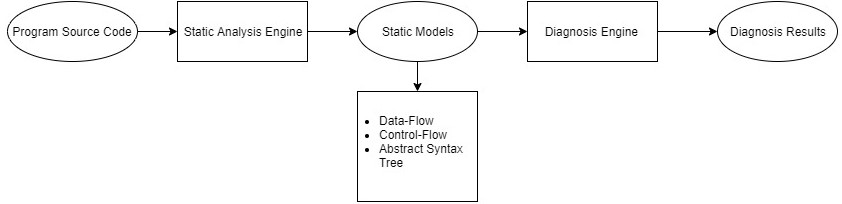
\includegraphics[width=1\textwidth]{Imgs/static_analysis.jpg}
    \caption{\label{fig:SysArch}System Architecture}
\end{figure}

The static analysis engine builds models by parsing the source code of the computer software and creates static models. The models are consist of abstract syntax trees.

The diagnosis engine analysis the models created by static analysis engine. By using the analysis results, it creates results of potential overflows. 

\section{STATIC ANALYSIS ENGINE}
The static analysis engine firstly parses the source code into tokens. After that, it creates abstract syntax tree by analysing statements and expressions. In this project, statements and expressions are limited with some types such as if statements, assign statements and while loops. Also data types are limited with primitive int and char types. Also stack arrays and pointers can be parsed by static analysis engine.

\begin{figure}[!htbp]
    \centering
    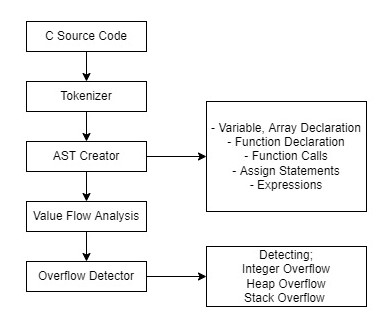
\includegraphics[width=0.8\textwidth]{Imgs/Structure.jpg}
    \caption{\label{fig:SysArch}System Architecture}
\end{figure}

\section{DIAGNOSIS ENGINE}
The diagnosis engine starts with value flow analysis. The statements inside the abstract syntax tree are executed at first. 

While this execution in progress, the overflow check occurs. For example, the expressions are tested before the execution if any overflow may occur. Also, array bound check and other type of buffer overflows are checked in this step.
\subsubsection{Integer Overflow Analysis}
In the design of the project, each expression are designed to return a result. And while calculating the result of the statements, overflow conditions may occur. That's why, at each result calculation, integer overflow analysis is done. 

The integer overflow in a program that is written with C language results in undefined behaviour. That's why, the overflow analysis is done before the statement executions or before calculating expression results.

\begin{figure}[!htbp]
    \centering
    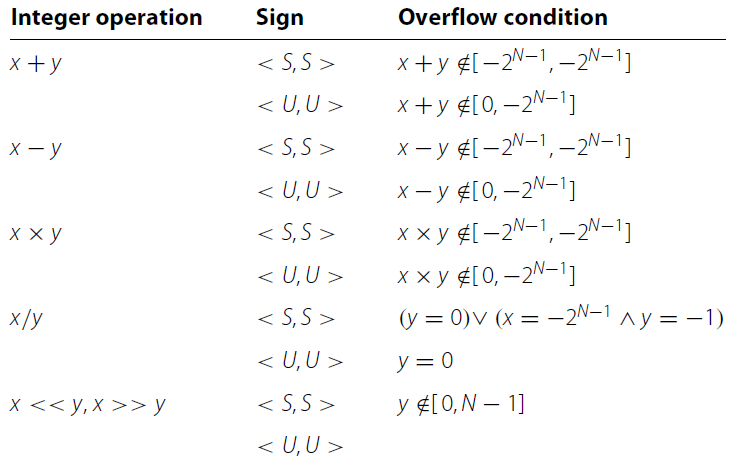
\includegraphics[width=0.8\textwidth]{Imgs/Integer_Overflow_conditions.png}
    \caption{\label{fig:SysArch}Integer Overflow Conditions}
\end{figure}

The figure 2.3 shows the overflow condition for integer operations. \cite{Three}

\subsubsection{Stack and Heap Overflow Analysis}
Stack and heap overflows are caused by accessing outside the bounds of the allocated area. That's why, the bound checking is the first criteria for stack and heap overflow analysis.

There are many unsafe Standard C Library and system data copy functions that can cause buffer overflow vulnerabilities. By using static analysis, it is not possible to detect overflows without analysing the source code. 

\begin{figure}[!htbp]
    \centering
    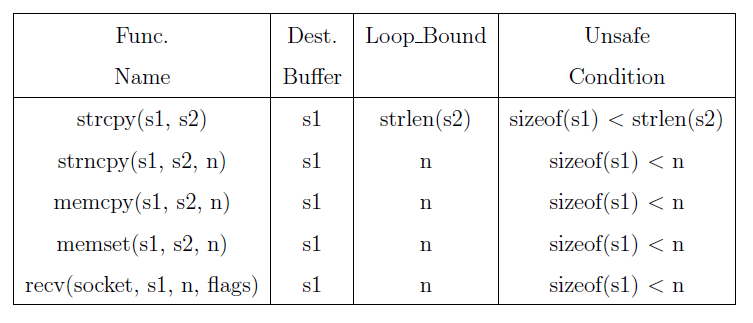
\includegraphics[width=0.8\textwidth]{Imgs/unsafefuncs.png}
    \caption{\label{fig:SysArch}The sample unsafe standard C library functions \cite{One}}
\end{figure}

In the figure 2.4, some sample of vulnerable standard C library functions are listed. The static analysis tools must be aware of these type of functions and analyse their parameters to detect buffer overflows.

\begin{figure}[!htbp]
    \centering
    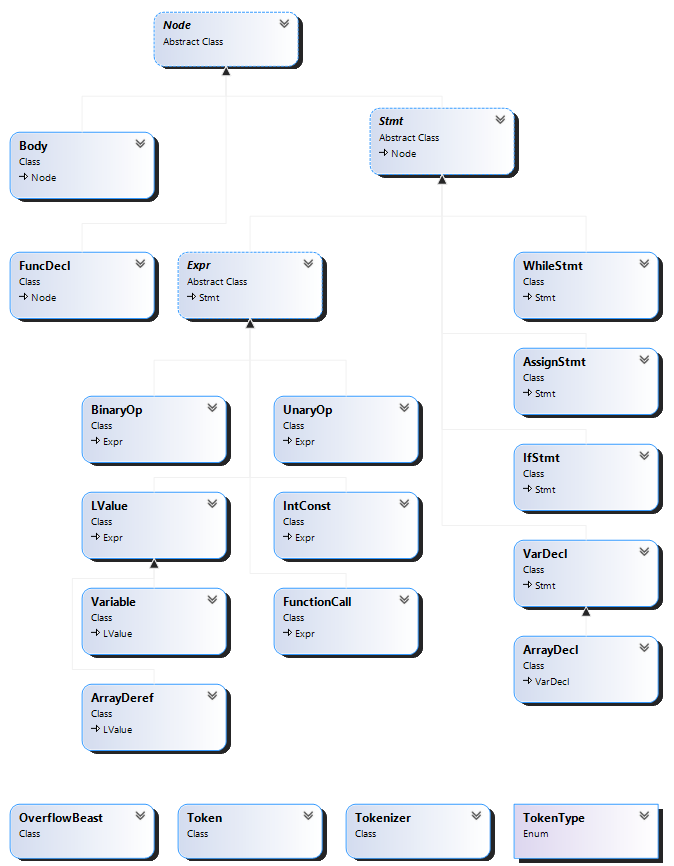
\includegraphics[width=1\textwidth]{Imgs/ClassDiagram2.png}
    \caption{\label{fig:ClassDiagram}Class Diagram}
\end{figure}

\clearpage

\section{REQUIREMENTS}

The project requirements are listed below:
\begin{itemize}
    \item The program shall be able to detect integer, stack and heap based overflow vulnerabilities.
    \item The program shall be able to detect overflows caused by vulnerable C library functions.
    \item The program will list errors in a Graphical User Interface.
    \item C# Language and libraries.
    \item Static analysis tools such as CppCheck for tests and comparisons.
    \item Microsoft Visual Studio IDE for creating GUI and developing the program.
    

\end{itemize}